In this report we show the numerical experiments. 
\subsection{Questions}
\begin{figure}[h]
	\centering
	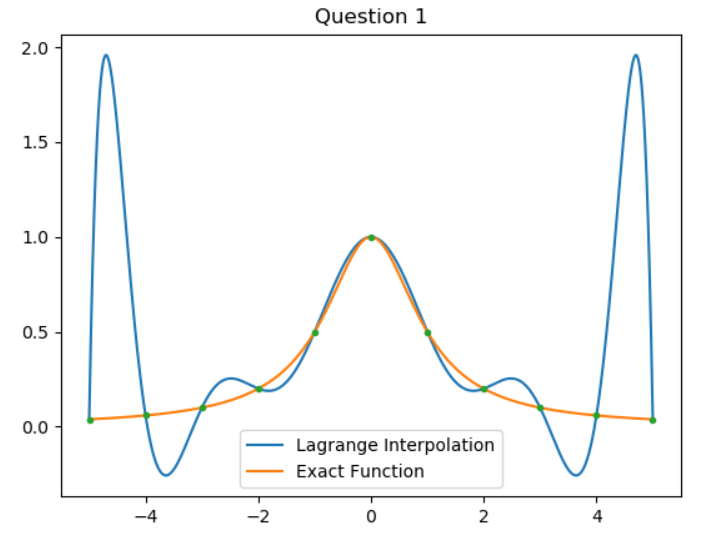
\includegraphics[scale=.5]{../fig/q1.png}
\end{figure}
\begin{figure}[h]
	\centering
	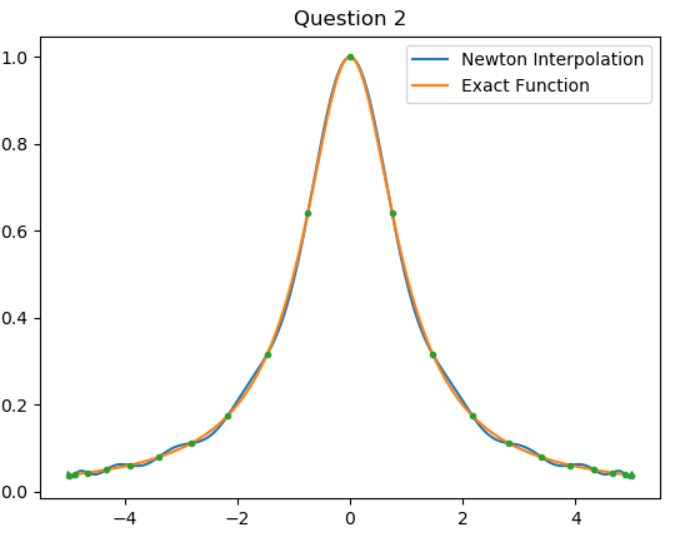
\includegraphics[scale=.5]{../fig/q2.png}
\end{figure}
\begin{figure}[h]
	\centering
	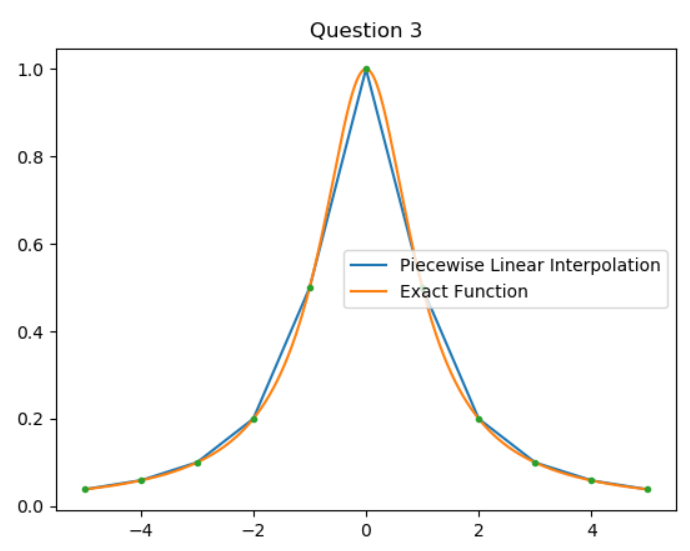
\includegraphics[scale=.5]{../fig/q3.png}
\end{figure}
\begin{figure}[h]
	\centering
	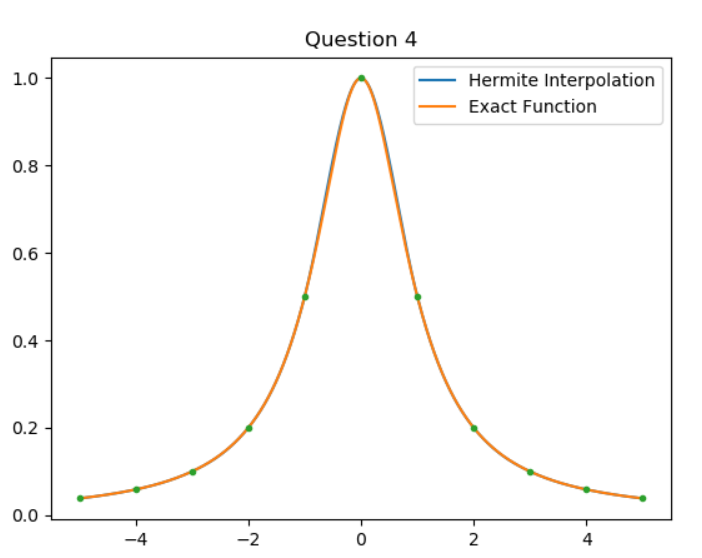
\includegraphics[scale=.45]{../fig/q4.png}
\end{figure}
\begin{figure}[h]
	\centering
	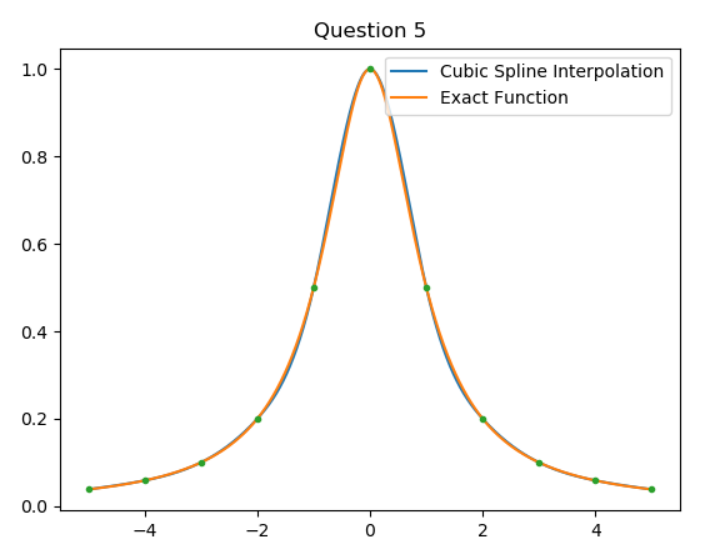
\includegraphics[scale=.45]{../fig/q5.png}
\end{figure}


We show several figures demonstrate the interpolation methods and results, corresponding to each question. Additionally, we compare the error between the Hermite method and cubic spline method. 
\begin{figure}[h]
	\centering
	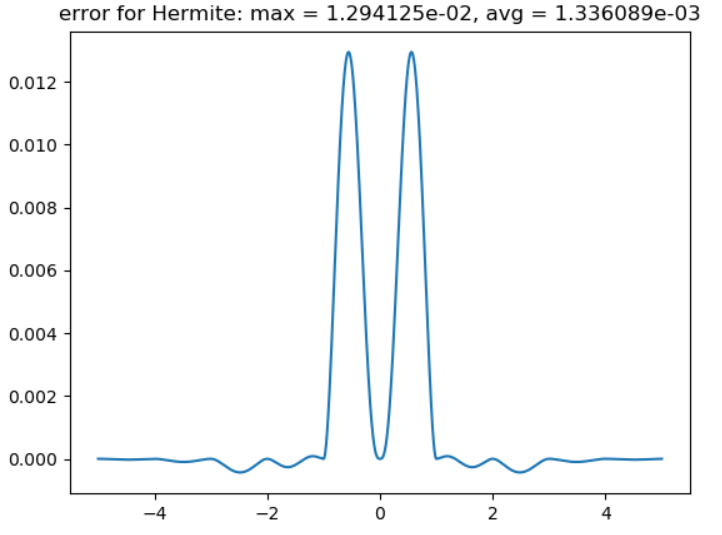
\includegraphics[scale=.3]{../fig/err.png}
	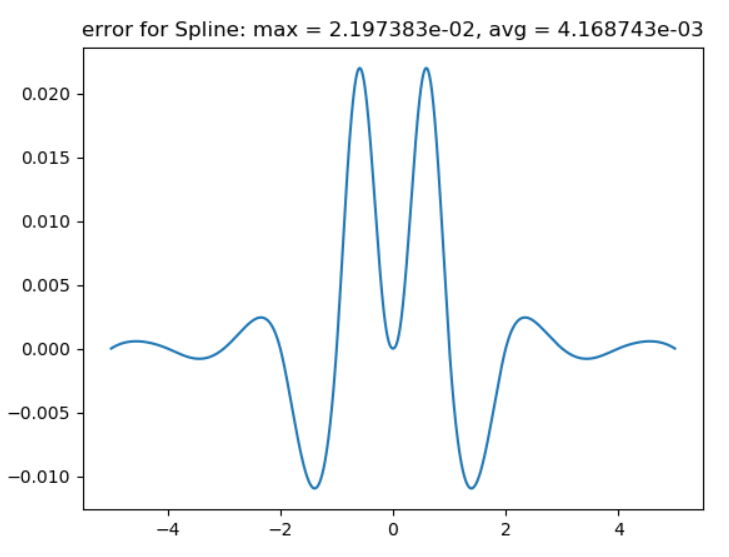
\includegraphics[scale=.3]{../fig/err5.png}
	\caption{The interpolation error of Hermite and Cubic spline methods.}
\end{figure}

\subsection{Discussions}

From the figure we can know that in this situation things are better when Hermite method is used. However, more condition like derivatives is required, which is laborious or even impossible to obtain in real application. So cubic spline meets the practical demand. 

Now we turn to the first two examples which uses the same global polynomial interpolation but with different node sets. They differs much as we see.  This is called Runge's phenomena. Ideally, this can be remedied by a good interpolation nodes set.
